
\documentclass[crop,tikz]{standalone}
\usepackage{hyperref}
\usepackage{amsmath}
\usetikzlibrary{decorations.pathreplacing}

\definecolor{presDark}{RGB}{39,1,136}
\definecolor{presDark2}{RGB}{87,80,149}
\definecolor{presLight}{RGB}{139,131,215}
\definecolor{presLight2}{RGB}{0,129,203}

\definecolor{presHighlight}{RGB}{215,50,50}

\begin{document}
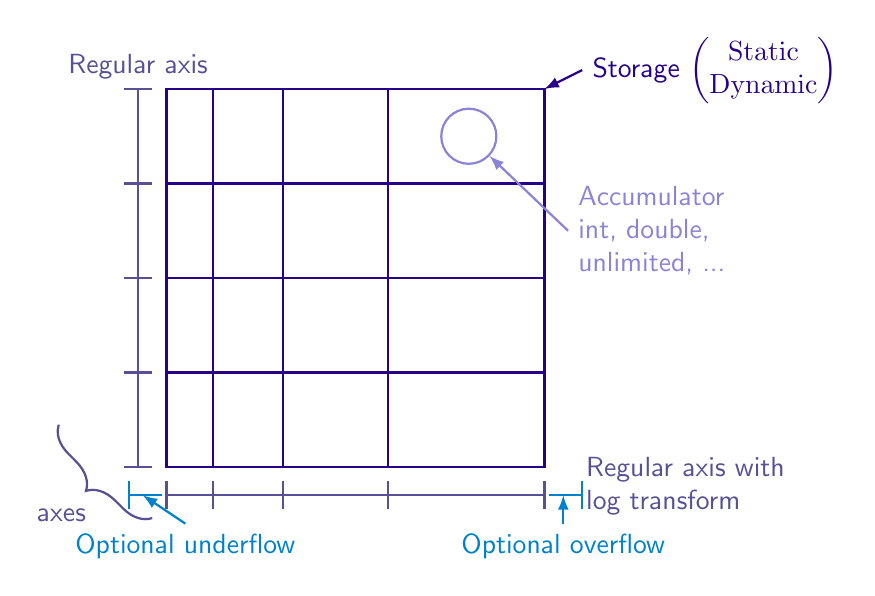
\begin{tikzpicture}[scale=1.2, font=\sffamily, every path/.style={thick}]

% Main grid
\draw [presDark] (-2,-2) rectangle (2,2);
\foreach \i in {-1,0,1} {
    \draw [presDark] (-2,\i) -- (2,\i);
}
\foreach \i in {-1.50465122, -0.76393202,  0.34370152} {
    \draw [presDark] (\i, -2) -- (\i, 2);
}
\draw [latex-, presDark] (2,2) -- (2.4,2.2) node [right] {Storage $\begin{pmatrix}\textrm{Static}\\ \textrm{Dynamic}\end{pmatrix}$};

% Left axis
\draw [presDark2] (-2.3,-2) -- (-2.3,2);
\foreach \i in {-2,-1,0,1,2} {
    \draw [presDark2] (-2.45,\i) -- (-2.15,\i);
}
\node at (-2.3,2) [above, presDark2] {Regular axis};

% Bottom axis
\draw [presDark2] (-2,-2.3) -- (2,-2.3);
\foreach \i in {-2.        , -1.50465122, -0.76393202,  0.34370152,  2.} {
    \draw [presDark2] (\i, -2.45) -- (\i, -2.15);
}
\node at (2,-2.2) [presDark2, right=.4cm, align=left] {Regular axis with\\log transform};

% Axes
\begin{scope}[xshift=-2.9cm, yshift=-2.3cm, rotate=45]
\draw [presDark2, decorate, decoration={brace,amplitude=10pt}, xshift=-4pt, yshift=0pt]
    (0.5,-0.7) -- (0.5,0.7);
\node at (-.3,0) [presDark2] {axes};
\end{scope}

% Overflow bin
\draw [presLight2] (2.05,-2.3) -- (2.4, -2.3);
\draw [presLight2] (2.4, -2.45) -- (2.4, -2.15);
\draw [presLight2, latex- ] (2.2, -2.3) -- (2.2, -2.6) node [below] {Optional overflow};

% Underflow bin
\draw [presLight2] (-2.05,-2.3) -- (-2.4, -2.3);
\draw [presLight2] (-2.4, -2.45) -- (-2.4, -2.15);
\draw [presLight2, latex- ] (-2.25, -2.3) -- (-1.8, -2.6) node [below] {Optional underflow};

% Accumulators
\node (accum) at (1.2,1.5) [circle, minimum width=.7cm, draw, presLight] {};
\draw [presLight, latex-] (accum) -- (2.25, .5) node [right, align=left] {Accumulator\\int, double,\\unlimited, ...};

\end{tikzpicture}
\end{document}
